\documentclass[aspectratio=169,12pt]{beamer}
\usefonttheme{serif}
\useinnertheme{default}
\useoutertheme{default}
\setbeamertemplate{navigation symbols}{}
\setbeamertemplate{footline}[frame number]

\usepackage[utf8]{inputenc}
\usepackage[T1]{fontenc}
\usepackage{lmodern}
\usepackage{tikz}
\usetikzlibrary{arrows.meta,positioning,calc,fit}
\usepackage{amsmath}
\usepackage{ragged2e}

\definecolor{wikiblue}{RGB}{51,102,204}
\definecolor{wikidark}{RGB}{32,33,34}
\definecolor{wikigray}{RGB}{84,89,93}
\definecolor{wikiborder}{RGB}{200,204,209}
\definecolor{wikibox}{RGB}{248,249,250}
\definecolor{wikibox2}{RGB}{234,236,240}
\definecolor{wikilightblue}{RGB}{238,243,255}

\setbeamercolor{normal text}{fg=wikidark,bg=white}
\setbeamercolor{title}{fg=wikidark}
\setbeamercolor{frametitle}{fg=wikidark,bg=white}
\setbeamercolor{structure}{fg=wikiblue}
\setbeamercolor{block title}{fg=wikidark,bg=wikibox2}
\setbeamercolor{block body}{fg=wikidark,bg=wikibox}
\setbeamercolor{alertblock title}{fg=wikidark,bg=wikibox2}
\setbeamercolor{alertblock body}{fg=wikidark,bg=wikibox}
\setbeamerfont{frametitle}{size=\large}
\setbeamerfont{block title}{size=\normalsize}
\setbeamertemplate{blocks}[rounded][shadow=false]

\tikzset{
  wikiarrow/.style={->, thick, draw=wikigray, >=Latex},
  wikistep/.style={
    draw=wikiborder,
    fill=wikibox,
    rounded corners=1.5pt,
    thick,
    align=center,
    text=wikidark,
    font=\scriptsize,
    minimum width=3.25cm,
    minimum height=0.82cm,
    inner sep=2.5pt
  },
  wikistephi/.style={
    draw=wikiborder,
    fill=wikilightblue,
    rounded corners=1.5pt,
    thick,
    align=center,
    text=wikidark,
    font=\scriptsize,
    minimum width=3.25cm,
    minimum height=0.82cm,
    inner sep=2.5pt
  },
  wikiboxnote/.style={
    draw=wikiborder,
    fill=wikibox,
    rounded corners=1.5pt,
    thick,
    align=left,
    text=wikidark,
    font=\scriptsize,
    inner sep=4pt,
    text width=4.15cm
  }
}

\begin{document}

\begin{frame}[t]{Article Generation Pipeline}
\hspace*{-0.035\textwidth}%
\begin{minipage}{1.07\textwidth}
\begin{columns}[T,totalwidth=\linewidth,onlytextwidth]
\column{0.55\linewidth}
\centering
\resizebox{\linewidth}{!}{%
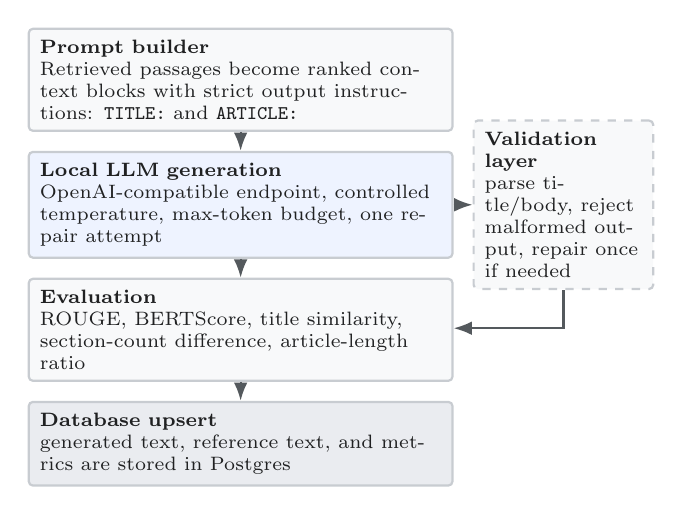
\begin{tikzpicture}[node distance=0.24cm]
  \node[wikiboxnote, text width=5.1cm] (p) {\textbf{Prompt builder}\\Retrieved passages become ranked context blocks with strict output instructions: \texttt{TITLE:} and \texttt{ARTICLE:}};
  \node[wikiboxnote, fill=wikilightblue, text width=5.1cm, below=of p] (g) {\textbf{Local LLM generation}\\OpenAI-compatible endpoint, controlled temperature, max-token budget, one repair attempt};
  \node[wikiboxnote, text width=5.1cm, below=of g] (e) {\textbf{Evaluation}\\ROUGE, BERTScore, title similarity, section-count difference, article-length ratio};
  \node[wikiboxnote, fill=wikibox2, text width=5.1cm, below=of e] (d) {\textbf{Database upsert}\\generated text, reference text, and metrics are stored in Postgres};
  \node[wikiboxnote, dashed, text width=2.0cm, right=0.24cm of g] (v) {\textbf{Validation layer}\\parse title/body, reject malformed output, repair once if needed};

  \draw[wikiarrow] (p) -- (g);
  \draw[wikiarrow] (g) -- (e);
  \draw[wikiarrow] (e) -- (d);
  \draw[wikiarrow] (g.east) -- (v.west);
  \draw[wikiarrow] (v.south) |- ($(e.east)+(0,0.02)$);
\end{tikzpicture}%
}
\column{0.42\linewidth}
\vspace*{-0.8cm}

\begin{block}{Runner behavior}
\scriptsize
\begin{itemize}
  \item single-article or batch execution
  \item schema creation for \texttt{generated\_articles}
  \item skip-existing logic from database state
  \item per-article error isolation for long runs
\end{itemize}
\end{block}

\vspace{0.04cm}
\begin{block}{Cost profile}
\scriptsize
Generation dominates runtime. Retrieval, prompt assembly, and database writes are much cheaper, while larger $k$ and larger token budgets mainly increase latency.
\end{block}

\vspace{0.04cm}
\begin{block}{Stored output}
\scriptsize
Each run persists the generated article together with the withheld reference text and evaluation metrics, enabling direct comparison across prompts, models, and retrieval settings.\\ With more project time, this can be used for improving the prompts/structure.
\end{block}
\end{columns}
\end{minipage}
\end{frame}

\begin{frame}[t]{Conclusion \& Future Work}
\vspace{-0.10cm}
\hspace*{-0.025\textwidth}%
\begin{minipage}{1.05\textwidth}
\begin{block}{Conclusion}
\justifying\scriptsize
The implemented system already provides a complete retrieval-to-generation baseline: it loads article metadata and reference text from Postgres, retrieves evidence from FAISS-indexed passages, builds a constrained prompt, generates a Wikipedia-style article draft with a local LLM, evaluates the result against the withheld reference article, and stores outputs plus metrics for reproducible comparison.
\end{block}

\vspace{0.08cm}
\begin{columns}[T,totalwidth=\linewidth,onlytextwidth]
\column{0.495\linewidth}
\begin{block}{What already works well}
\scriptsize
\begin{itemize}
  \item end-to-end reproducible pipeline
  \item explicit grounding in retrieved passages
  \item lexical, semantic, and structural evaluation
  \item resume-friendly batch processing via upserts
\end{itemize}
\end{block}

\column{0.495\linewidth}
\begin{block}{Future work}
\scriptsize
\begin{itemize}
  \item section-wise RAG instead of single-shot generation
  \item better topic inference and query expansion
  \item stronger redundancy reduction before prompting
  \item tuning of $k$, prompt length, and model choice
  \item richer factuality checks beyond overlap metrics
\end{itemize}
\end{block}
\end{columns}

\vspace{0.04cm}
\begin{alertblock}{Takeaway}
\scriptsize
The strongest next gains will likely come from better retrieval structure and more controlled generation rather than from rebuilding the pipeline itself.
\end{alertblock}
\end{minipage}
\end{frame}

\end{document}
